\subsection{Background}


The city of Madison presents a significant opportunity for the implementation of electric vehicle (EV) charging infrastructure. There are a plethora of available parking lots in the city, each of which has the potential to serve a specific region and meet the demands of local parking needs. In particular, the downtown and campus areas of Madison exhibit a higher density of parking lots, reflective of the increased demand for parking in these areas. In light of this, it is assumed that all EV charging stations will be situated within existing parking lots, as EVs typically utilize their parking time for charging. Furthermore, indoor parking lots provide an optimal environment for EV charging, as their construction design can facilitate the maintenance of desirable temperature and voltage levels, which are crucial for effective battery charging.

To simplify the model, the city of Madison has been divided into sixteen equally-sized areas, with two parking lots assumed to cover each area. This model can be easily adapted to account for additional parking lots and different area divisions, providing a flexible framework for the implementation of EV charging infrastructure in Madison.
\begin{figure}[t]
    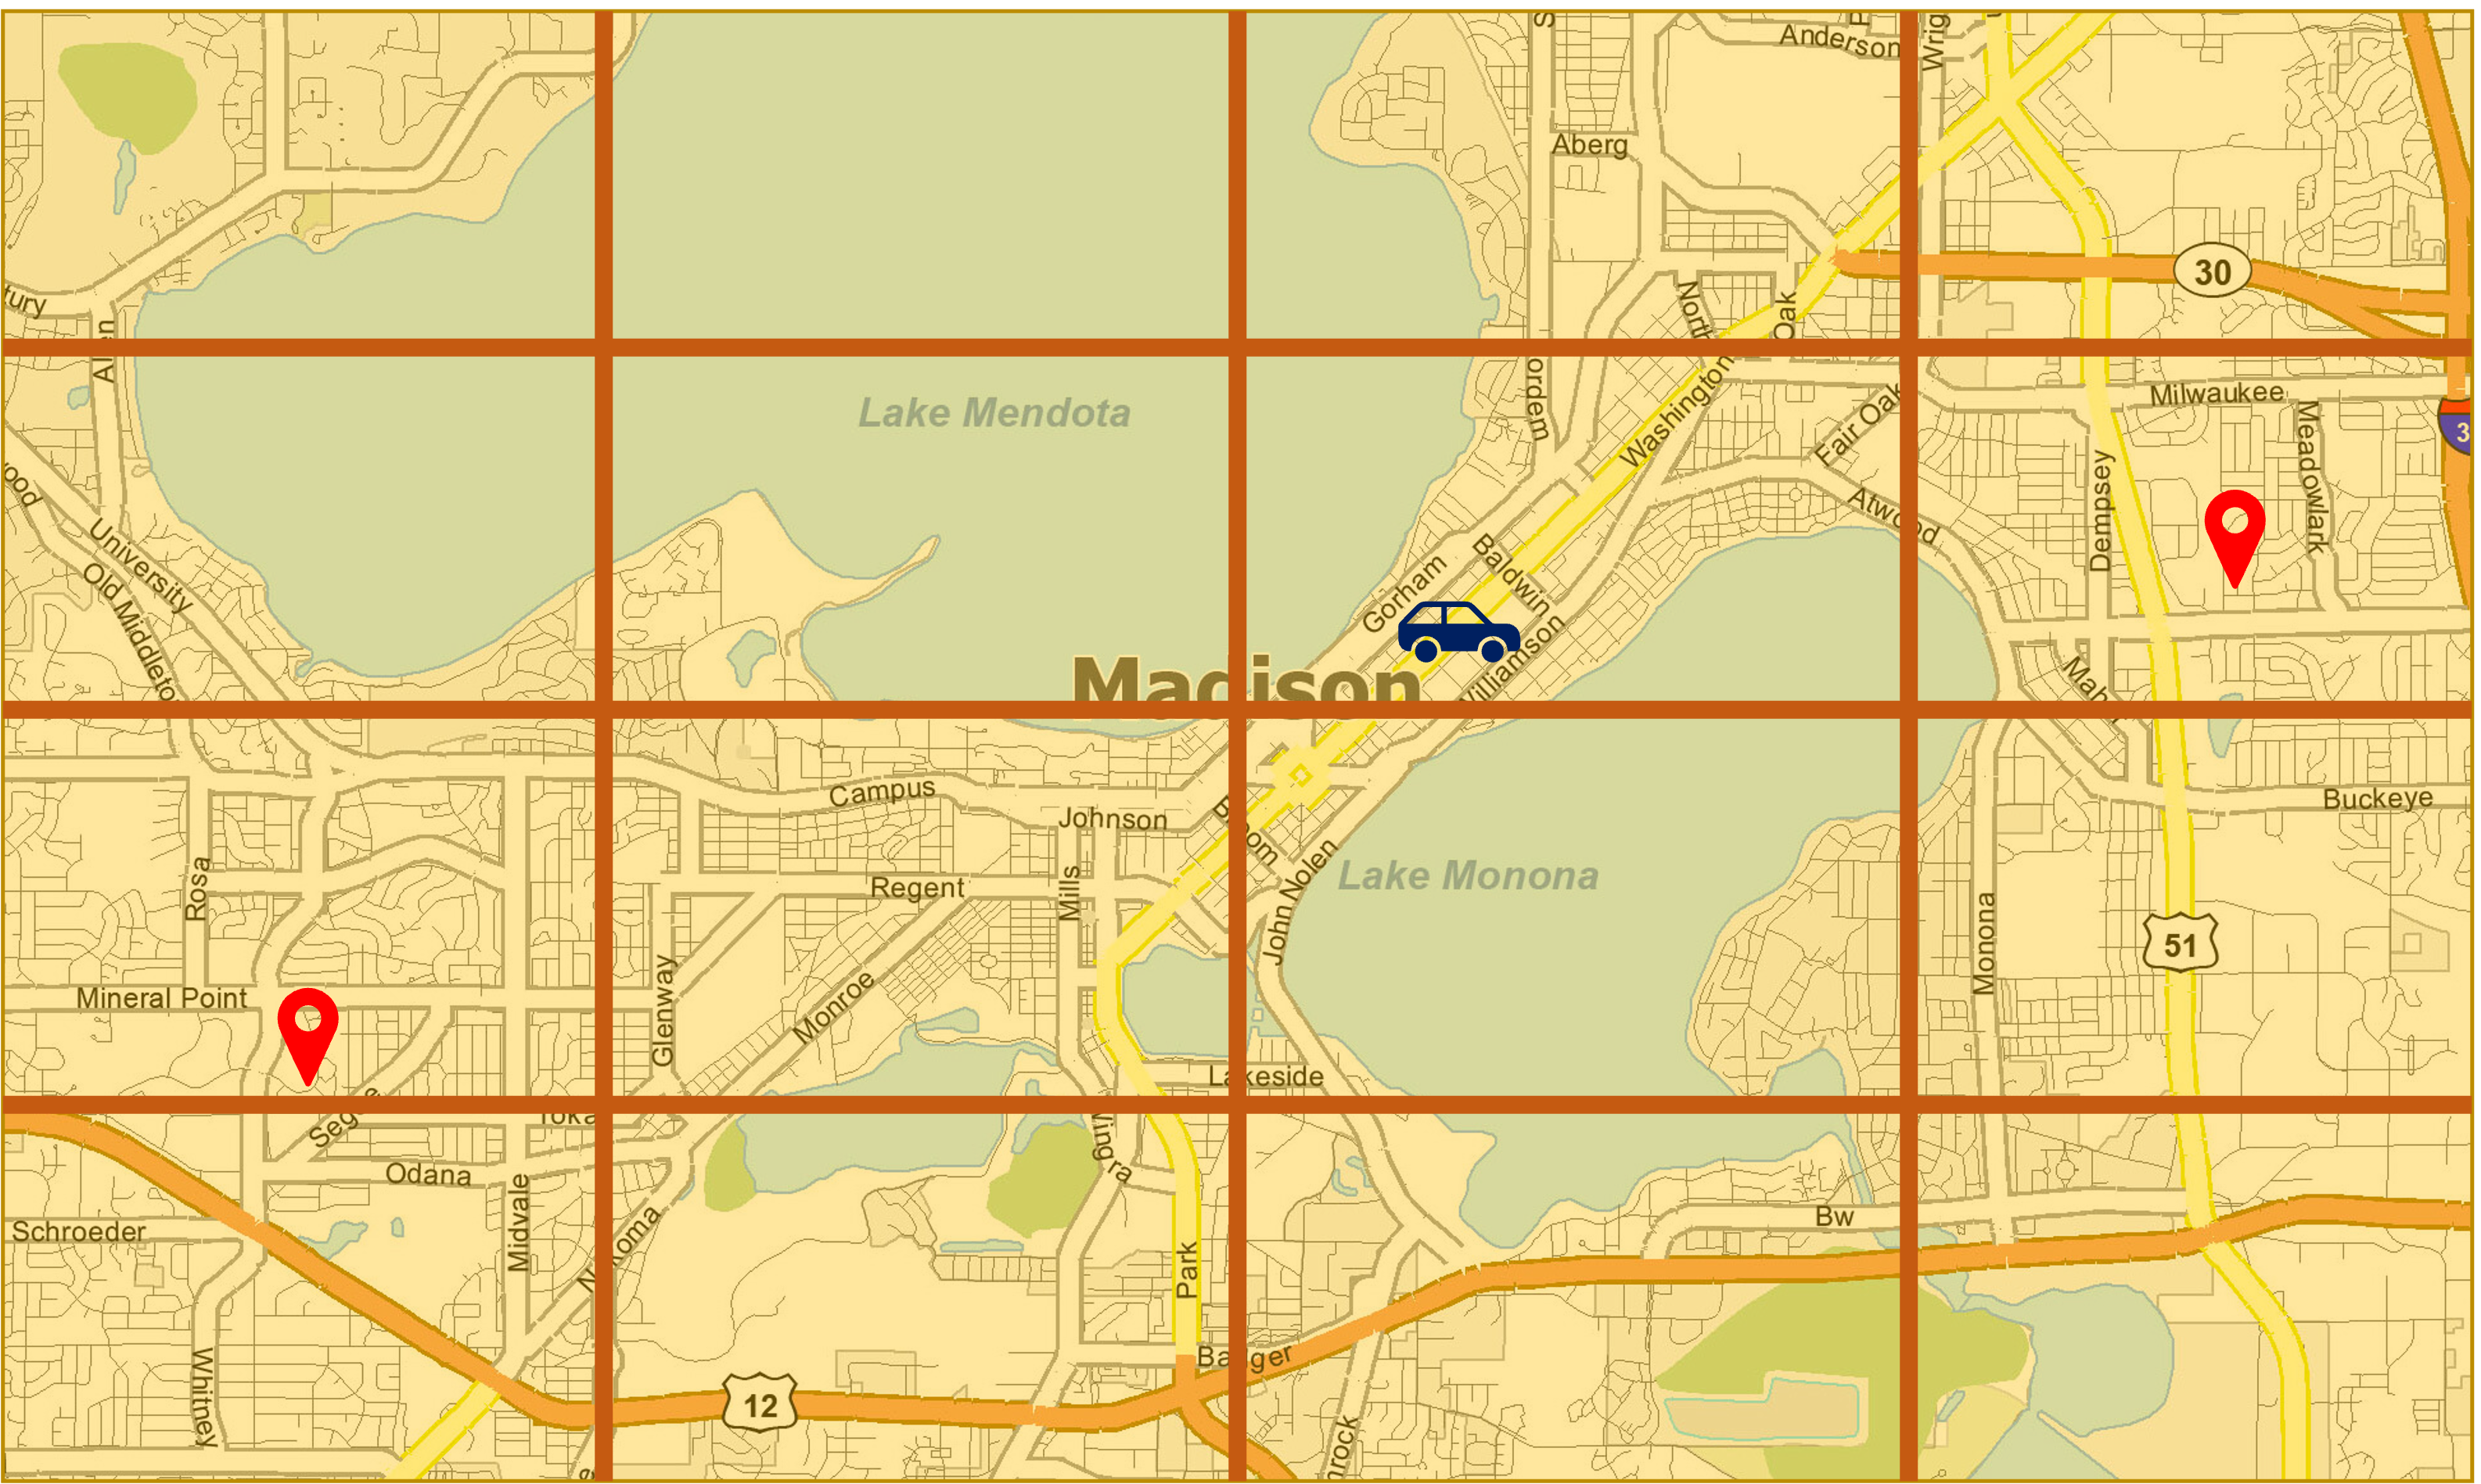
\includegraphics[width = 0.8\textwidth]{figure/madison.png}
    \centering
    \caption{The city division and parking lots assumption}
    \label{fig:madison}
    \end{figure}



\subsection{Model Overview}
In order to accurately simulate the scenario of EV charging infrastructure implementation in Madison, a comprehensive model was developed that is divided into three key components: Data Generation, Drivers' Choice, and Parking Simulation. The flowchart~\ref{fig:flowchart} provided illustrates the structure of the model and the inter-dependencies between the various components.

Given the paucity of available data, the Data Generation component of the model is crucial in generating synthetic data to be used in the subsequent stages of the model. As such, the validity of the results obtained is contingent upon the quality of the data generated. However, when real-world data becomes available, it can be easily integrated into the model by modifying the Data Generation component, thereby enabling the generation of results that are reflective of reality.

\begin{figure}[t]
    \includegraphics[width = 0.8\textwidth] {figure/flowchart.png}
    \centering
    \caption{The overall structure of the model}
    \label{fig:flowchart}
    \end{figure}



\subsection{Model Details}
\subsubsection{Data Generation}
\textbf{Scenario}: In our model, we consider parking and charging event happening in different scenarios: normal days and Game days. During normal days, we assume that the traffic flow is even over all regions. During Game days, because the high demand of parking near the stadium, there will be a certain period of time in a day that one parking lots will have heavy traffic. 

For simplicity, we set up a uniform distribution of incoming traffic flow on normal days. Namely, the drivers will arrive at the parking lot with equivalent time gap. While for Game days situation, we let 80\% of traffic flow arrives during 10\% of the time in a day to simulate the situation. 

\textbf{Price}: In our model, we assumed price is the one of the key factor influencing the driver's decision of which parking lot to go. The price can be a fixed number, or be selected dynamically within a certain range. For Game days scenario, we applied a \textbf{Gameday multiple} to modify the price to see the influence. 

\textbf{Spots}: Spots refer to the available chargers in certain parking lots, and we also considered this as one of the factors that will influence the driver's decision. We assumed under the budget, there will only be limited number of available chargers altogether to be implemented in the city. In most of our experiments, this number is set to be 20. 

\textbf{Distance(Pref)}: Distance refers to the distance from the parking lot to the driver's desired destination. Usually, people intends to park as close as possible to their destination, so this factor can also be understood as the preference value of the parking lots by each driver. The smaller the distance, the more preferable the parking lot. In our experiment, we generate this value from uniform distribution in certain range. 

\subsubsection{Choice Model}

The driver's choice can be viewed as a decision over utility of each parking lots. We intrdouced the well-know Cobb-Douglas utility function to simulate the decision process of each driver. With the input of price, spots, and distance, each driver will have an utility value of each parking lots. Based on the corresponding utility value, the driver will make a probability-based choice: The higher the value, the more possible the driver will choose certain parking lot. The reason we introduce the probability choice model is to simulate the possible unexpected decisions from drivers. 

More precisely, we have
utility function designed as
$$
\mu_{d_i}(l) = P^{\alpha} S^{\beta} D^{\gamma}
$$

where $d_i$ represents the $i$ th driver, $l$ represents the selected parking lot, $P$ represents Price, $S$ represents Spots, $D$ represents Distance. $\alpha, \beta, \gamma$ are parameters tuned for simulation. 

The decision function is 
$$
\mathbb{P}_{d_i}(l) = Bin(1, \mu_{d_i}(l))
$$

Based on the current position of each driver and decision made from the model, we can generate the incoming flow to each parking lots, which gives us the Inflow Data. 


\subsubsection{Parking Simulation}
The parking simulation can be divided into several small process: entering process, charging process, and queue process.

\paragraph{Entering Process}
When the driver arrives a certain parking lot, he/she may find two different situations: the parking lot does have available spot right now, or the parking lot is full and there's a queue for waiting. 

If there is an available spot, the driver will enter the lot and continue to charging process. If not, he/she has to join the queue. 

\paragraph{Charging Process}
After successfully entering the parking lot, the driver will start the charging process right away. We neglect the time gap for finding a specific spot, as this is not the main concern of the model. 

The charging time will depend on the current battery level of the car, therefore it varies from driver to driver. To simulate this situation, we applied a uniform distribution on determining the charging time. 

\paragraph{Queue Process}
If the driver didn't enter the parking lot and join the queue, then he/she must take the following procedure. 

The driver is supposed to stay at least for one time unit, and his/her patience is measured by the \emph{stay probability}. After each time unit, the driver's stay probability will decrease center amount, and once the stay probability goes under the threshold, the driver will leave the queue system and is designed to not come back. 

For each time unit, the driver will try to enter the parking lot. Because after each time unit, there will be some drivers finish charging, therefore there will be available spots open for the next driver. The entering rule follows first come, first serve, which means those who entered the queue system earlier and didn't leave will have priority to enter the system. 

Say the threshold is $p$, the decreasing amount is $\delta_p$, then the algorithm will be 

\begin{algorithm}
\caption{Driver Queue}
\label{alg:entry}
\begin{algorithmic}[1]
\If{$P_{stay} > p$}
\If{$Spot > 0$}
\State Enter System
\State Queue \textbackslash Driver
\Else
\State $P_{stay} \gets P_{stay} - \delta_p$
\EndIf
\EndIf
\end{algorithmic}
\end{algorithm}

\subsection{Evaluation Model}
Our evaluation model considers both the driver side and the designer side. For the driver, the rate of successful service, demand-meet of preference, and the price of charging are the primary considerations. For the designer, the occupancy rate of the chargers is the primary consideration. We use a satisfaction adjustment coefficient $\theta$ to balance the emphasis between the driver side and the designer side. The efficiency rate of chargers can also affect the balance between the two sides.

If the efficiency rate of chargers is above a certain threshold, such as 75\%, we prioritize driver satisfaction. By balancing the preferences of drivers and designers, our model can provide valuable insights for the development of EV charging infrastructure.